\subsection{CFL widths from mass conservation}
Hematocrit measures proportion of volume of red blood cells (RBC) to total 
blood volume (RBC and plasma) \cite{BillettHct}. Cell volume fraction or tube 
hematocrit $H_t$ is calculated as:
\begin{equation} \label{eq:tube_hct_vol}
H_t = \frac{N_c V_{eff}}{V_t}
\end{equation}
where $N_c$ is the number of RBCs in the tube volume $V_t = \pi R^2 L$, $R$ is 
the tube radius, and $L$ is the tube length \cite{MICC:MICC56}.

An empirical relation between $H_t$ and $H_d$ is given by:
\begin{equation} \label{eq:tube_hct_emp}
\frac{H_t}{H_d} = H_d + (1 - H_d) \left (1 + 1.7e^{-0.35D} - 0.6e^{-0.01D} 
\right)
\end{equation}
where $D$ is the tube diameter in micrometers, and discharge hematocrit $H_d$ 
is equal to systemic hematocrit \cite{lamkin2004impact}.

Since systemic hematocrit in both cases (non-bifurcating and bifurcating flow) 
is the same, $H_t$ is the same according to Eq. \ref{eq:tube_hct_emp}. Since 
$V_t$ is the same due to constant vessel diameter, $N_c$ assumed (?) to be the 
same, $V_{eff}$ must be the same (Eq. \ref{eq:tube_hct_vol}).

Ignoring gravity effect and assuming symmetry, we need to find a egg / ellipse 
shaped graph with the same area as the circle in non-bifurcating flow.

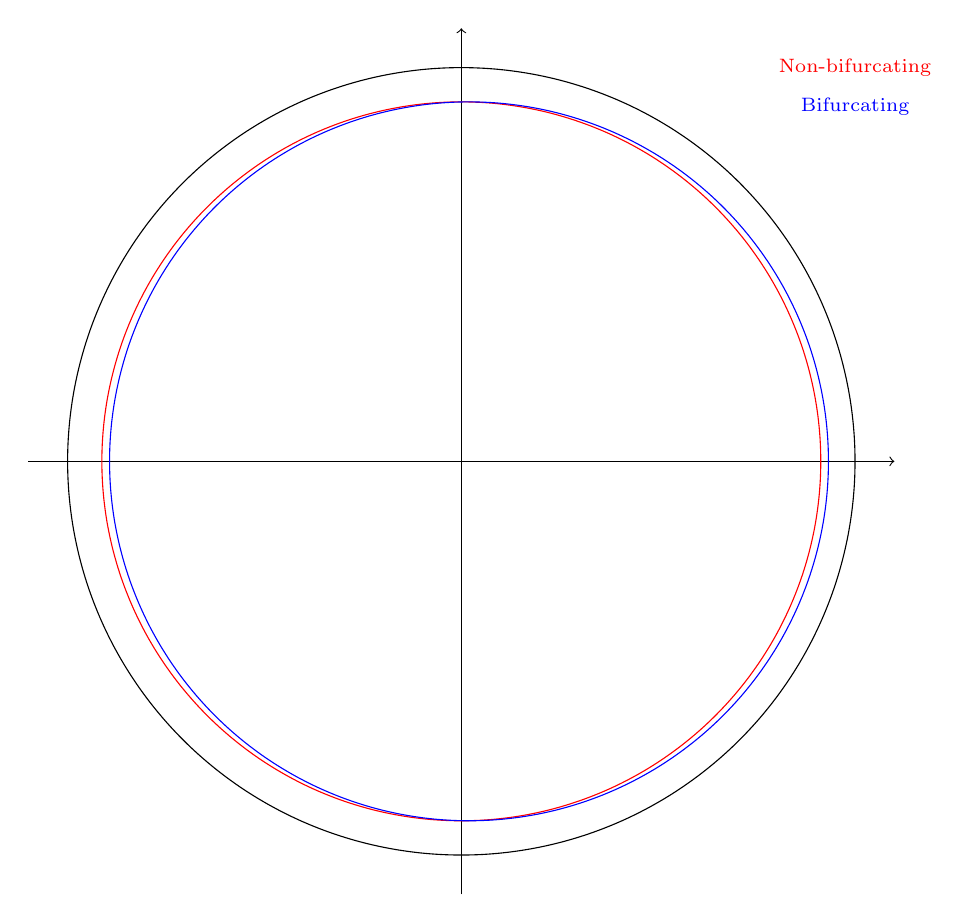
\begin{tikzpicture}[scale=0.1]
\draw[->] (-55,0) -- (55,0);
\draw[->] (0,-55) -- (0,55);
\draw node [red] at (50,50) {\scriptsize{Non-bifurcating}};
\draw node [blue] at (50,45) {\scriptsize{Bifurcating}};
\draw[color=black,domain=0:2*pi,samples=200,smooth] plot (xy polar
cs:angle=\x r,radius= {50});    %r = angle en radian
\draw[color=red,domain=0:2*pi,samples=200,smooth] plot (xy polar
cs:angle=\x r,radius= {45.65});    %r = angle en radian
\draw[color=blue,domain=0:2*pi,samples=200,smooth] plot (xy polar
cs:angle=\x r,radius= {0.975*cos(\x r) + (45.65^2-0.975^2*sin(\x 
r)^2)^0.5});    %r = %angle en radian
\end{tikzpicture}

\paragraph{Assumptions:}
Define normal CFL width as mean of inner and outer CFL width.
\begin{equation}
NCFL_{normal} = \frac{NCFL_{inner} + NCFL_{outer}}{2}
\end{equation}